\section{Method}

\begin{frame}
	\frametitle{Preparation: feature extraction}
	Apply "compute descriptors" tool from \alert{University of Surrey} with the following parameters:
	\begin{center}
		\textbf{-hesaff -sift -noangle}
	\end{center}
	\textbf{hesaff}: Scale and Affine invariant interest point detector\\
	\textbf{sift}: use Scale Invariant Feature Transform (SIFT) descriptor\\
	\textbf{noangle}: no angle estimation
\end{frame}

\begin{frame}
	\frametitle{Preparation: feature extraction}
	\begin{center}
	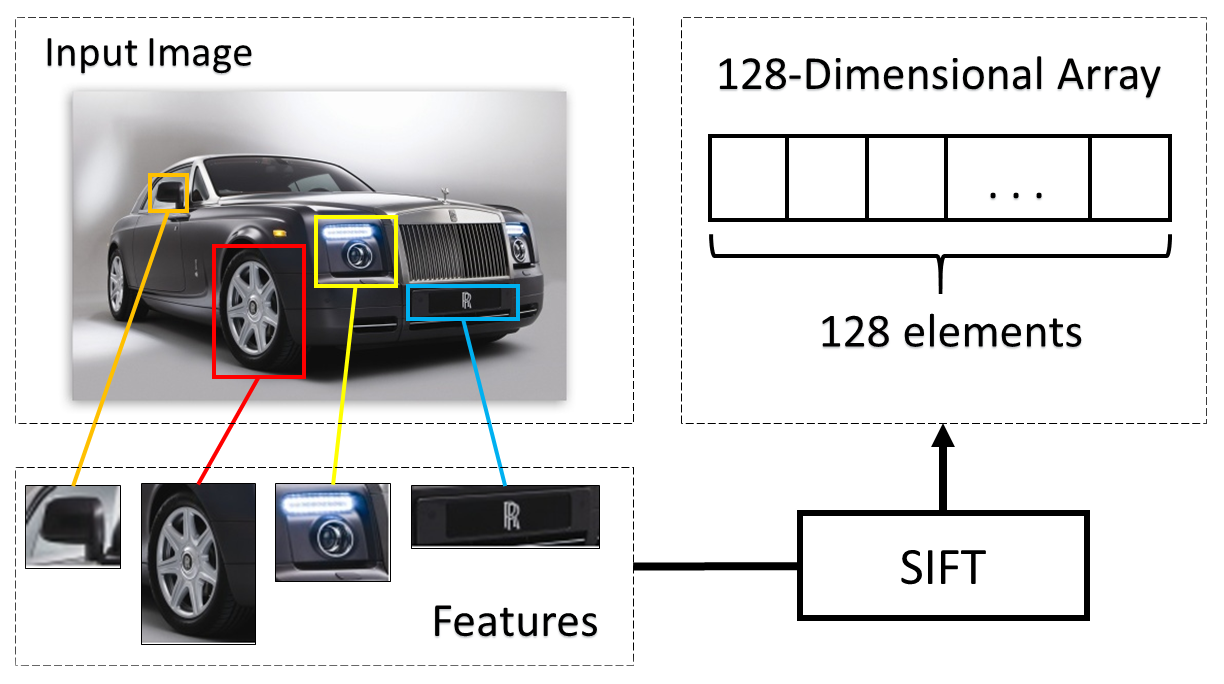
\includegraphics[width=\textwidth]{images/feature_extraction2.png}
	\end{center}
\end{frame}

\begin{frame}
	\frametitle{Preparation: codebook building}
	Use \textbf{approximate k-Means} to cluster all features to \textbf{1M} clusters
	\begin{itemize}
		\item Use \alert{FASTANN} and \alert{FASTCLUSTER} libraries \footcite{Muja, M. and Lowe, D.
Fast approximate nearest neighbours with automatic algorithm configuration
Proceedings of the International Conference on Computer Vision Theory and Applications (2009)} \footcite{Philbin, J. , Chum, O. , Isard, M. , Sivic, J. and Zisserman, A.
Object retrieval with large vocabularies and fast spatial matching
Proceedings of the IEEE Conference on Computer Vision and Pattern Recognition (2007)}
		\item \alert{Philbin et al.} shows that \textbf{1M} dictionary size produce best performance on \alert{Oxford Building} dataset
		\item Run with \textbf{50} iterations
	\end{itemize}
	Each image is presented by a \textbf{1M-dimensional} vector
\end{frame}

\begin{frame}
	\frametitle{Preparation: codebook building}
	\begin{center}
	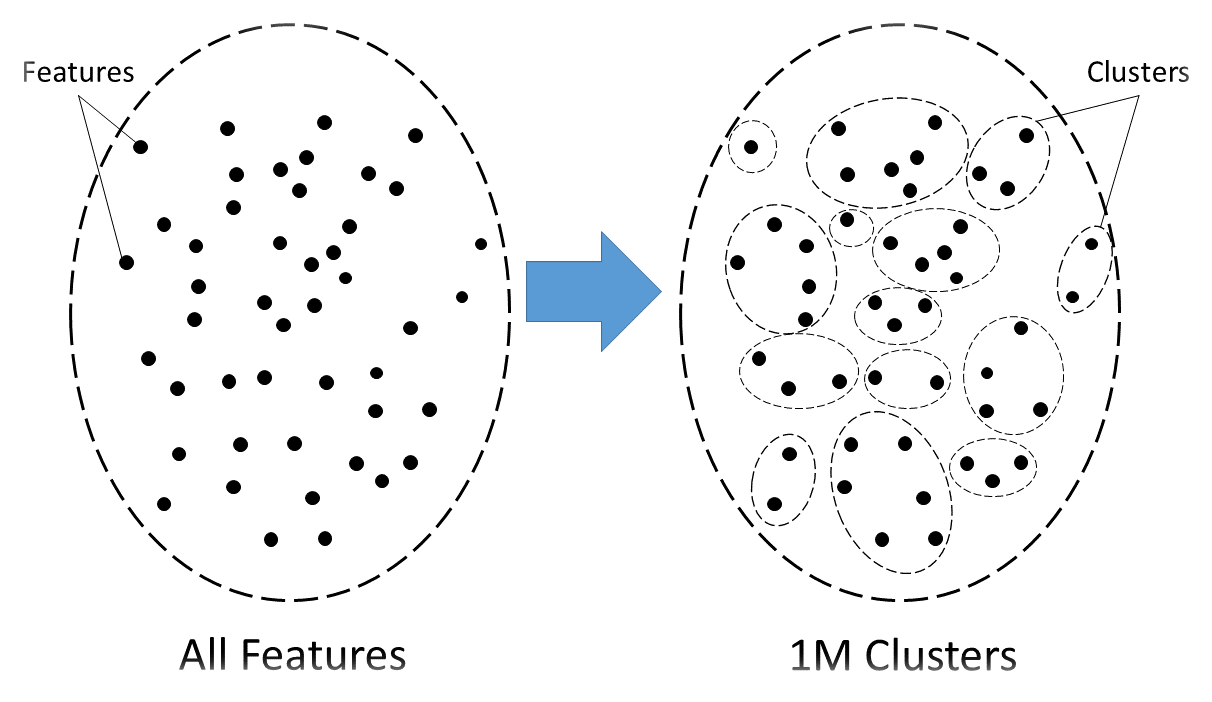
\includegraphics[width=\textwidth]{images/cluster2.png}
	\end{center}
\end{frame}

\begin{frame}
	\frametitle{Preparation: quantization (soft assignment)}
	\textbf{Soft assignment:} Each \textbf{128-dimensional} feature vector is reduced to \textbf{3-dimensional} by looking for its \textbf{3 nearest visual words}\\
	Each of the \textbf{nearest visual words} is assigned with \alert{weight}:
    \begin{equation*}
    	weight = exp(-\frac{d^2}{2\delta^2})
    \end{equation*}
\hspace{4ex} $d = $ distance from feature vector to cluster centroid

\hspace{4ex} $\delta^2 = 6250$\\

    All weights are added to their corresponding visual word in the \textbf{1M-dimensional} representation of the image
\end{frame}

\begin{frame}
	\frametitle{Preparation: quantization (natural soft assignment)}
	Use \textbf{natural soft assignment} to increase accuracy. 2 steps:\\\\
	\textbf{1. Detection of repetitive structures}:
	\begin{itemize}
		\item ${(x_{i},s_{i},d_{i})}$ is feature at location $x_{i}$, scale $s_{i}$, descriptor $d_{i}$
		\item 2 features are connected if
		\begin{enumerate}
			\item $L2$ distance $|x_{i}-x_{j}| < c(s_{i}+s_{j})$
			\item ratio $\sigma$ of 2 features is in $0.5 < \sigma < 1.5$
			\item 2 features share at least one common visual word
		\end{enumerate}
	\end{itemize}
	Find connected components of features. The detected components are called repttiles.
	
\end{frame}
	
\begin{frame}
	\frametitle{Preparation: quantization (natural soft assignment)}
	\textbf{2. Weight calculation for each visual word in an image:}\\\\
	$w_{id}$: weight of visual word i in image d\\
	$k_{f}$: number of nearest visual words we consider for feature f\\
	$V_{f}:$ set of indices of the $k_{f}$ nearest visual words to feature f
	\begin{equation*}
		w_{id}=\sum\limits_{f \in F_{d}} \sum\limits_{k=1}^{k_{f}}1[V_{f}(k)=i]\frac{1}{2^{k-1}}
	\end{equation*}
	where the indicator function $1[V_{f}(k)=i]$ equals to 1 if visual word i is at position k of $V_{f}$
	\begin{equation*}
		k_{f}=\left \lceil{k_{max} \frac{\log{\frac{n_{d}+1}{m_{f}}}}{max_{f \in F_{d}}\log{\frac{n_{d}+1}{m_{f}}}} }\right \rceil 
	\end{equation*}
	where $m_{f}$ is the number of features in the repttile of f
\end{frame}

\begin{frame}
	\frametitle{Preparation: quantization}
	\begin{center}
	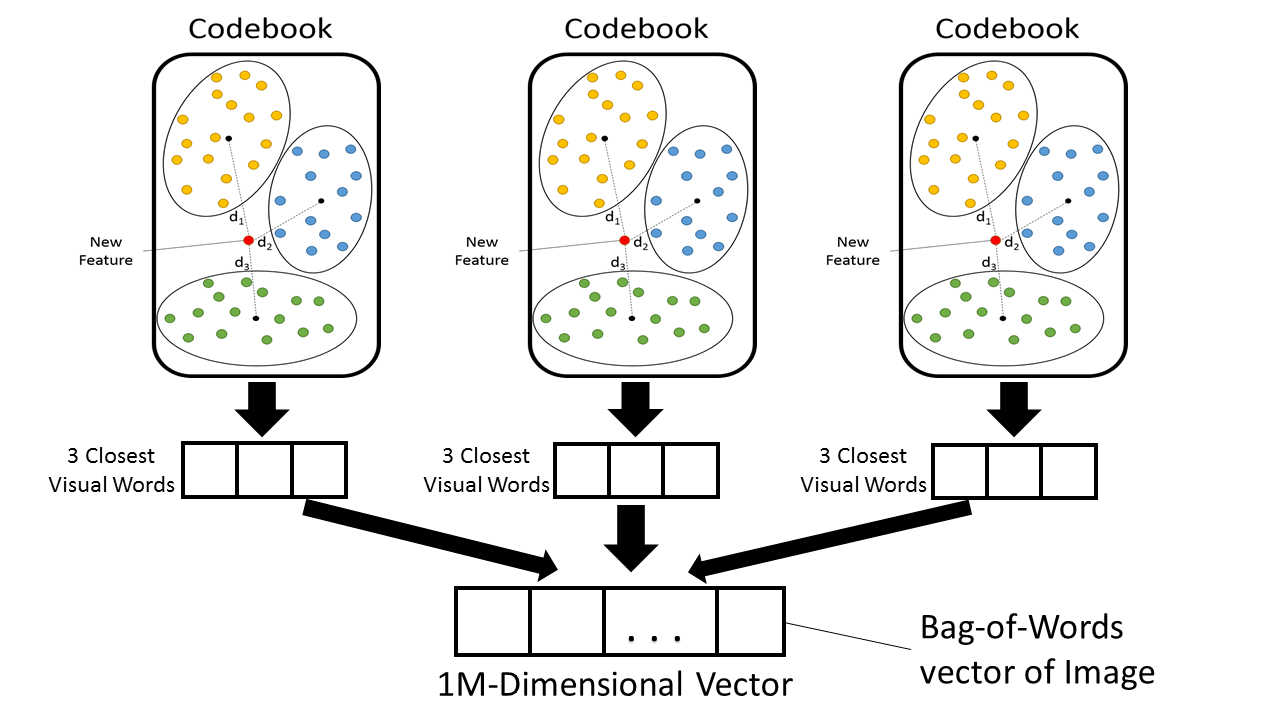
\includegraphics[width=\textwidth]{images/quantization.png}
	\end{center}
\end{frame}
